\documentclass{article}

\usepackage[ngerman]{babel}										% Statt german, \autoref zeigt damit "Abbildung x" an
\usepackage{graphicx}											% Graphiken einbinden
\usepackage[left=3cm,right=3cm,top=3cm,bottom=3cm]{geometry}	% Abstände zu den Papierrändern
\usepackage[utf8]{inputenc}										% Zeichenkodierung
\usepackage{mathtools}											% Stellt Mathe-Umgebung bereit
\usepackage{float}												% Improves floating elements
\usepackage{lmodern}											% Andere Schriftart (bessere Druckbarkeit)
\usepackage{pdfpages}											% Einbinden von PDF-Dokumenten
\usepackage{fancyhdr}											% Fancy Headers / Footers
\usepackage{listliketab}										% Lists with tab stops
\usepackage{setspace}											% Anpassung von Zeilenabständen
\usepackage{siunitx}											% Korrekte Darstellungen von Einheiten (\SI{1.5}{\milli\volt})
\usepackage{hyperref}   										% Objekte referenzieren (\autoref)
\usepackage{subcaption}
\usepackage{listings}
\usepackage{tikz}

% dark mode
%\usepackage{xcolor}			
%\pagecolor[rgb]{0,0,0}
%\color[rgb]{1,1,1}

\setlength{\parindent}{0em}										% Keine Einrückung bei Absatzbeginn
\setlength{\parskip}{1em}										% Dafür vert. Abstand zw. Absätzen

\renewcommand{\arraystretch}{1.2}								% Verzeichnisse kompakter darstellen

\newcommand{\tbf}{\textbf}										% Shortcut für fetten Text

\makeatletter
\g@addto@macro\bfseries{\boldmath}								% \mathbf nicht im Inhaltsverzeichnis darstellen
\makeatother

\pagestyle{fancy}												% Benutzung von fancyhdr
\sisetup{
	locale = DE,
	per-mode=fraction,
	fraction-function=\tfrac,
	binary-units = true
	}

\DeclareSIUnit{\belmilliwatt}{Bm}
\DeclareSIUnit{\dBm}{\deci\belmilliwatt}

\DeclareSIUnit{\belcarrier}{Bc}
\DeclareSIUnit{\dBc}{\deci\belcarrier}

\DeclareSIUnit{\belvolt}{BV}
\DeclareSIUnit{\dBV}{\deci\belvolt}

\DeclareSIUnit{\Bit}{Bit} % bits 

\usepackage{xcolor}

\definecolor{codegreen}{rgb}{0,0.6,0}
\definecolor{codegray}{rgb}{0.5,0.5,0.5}
\definecolor{codepurple}{rgb}{0.58,0,0.82}
\definecolor{codeblue}{rgb}{0,0,0.92}
\definecolor{backcolour}{rgb}{0.95,0.95,0.92}

\lstdefinestyle{codestyle}{
    backgroundcolor=\color{backcolour},   
    commentstyle=\color{codegreen},
    keywordstyle=\color{codeblue},
    numberstyle=\color{magenta},
    stringstyle=\color{codepurple},
    basicstyle=\ttfamily\footnotesize,
    breakatwhitespace=false,         
    breaklines=true,                 
    captionpos=b,                    
    keepspaces=true,                 
    numbers=left,                    
    numbersep=5pt,                  
    showspaces=false,                
    showstringspaces=false,
    showtabs=false,                  
    tabsize=2
}

\lstset{style=codestyle}
\lhead{}
\rhead{}

% anpassen!
\chead{Digitaltechnick - Praktikum 3}
\lfoot{13.05.2020}
\cfoot{Loïc Fernau, Niklas Bammann}

\rfoot{Seite \thepage}

\usepackage{titlesec}
\titlespacing\section{0pt}{12pt plus 4pt minus 2pt}{0pt plus 2pt minus 2pt}
\titlespacing\subsection{0pt}{0pt}{0pt}
\titlespacing\subsubsection{0pt}{12pt plus 4pt minus 2pt}{0pt plus 2pt minus 2pt}


\begin{document}
	% Titelseite anpassen
	%\includepdf[pages={3}]{pdf_ext/.pdf}

 	\begin{titlepage}
 		\begin{flushright}
			
\includegraphics[width=0.5\textwidth]{img/title.png}\\[2cm]
		\end{flushright}
		
		\begin{center}
			%\textsc{\LARGE Hochschule für angewandte Wissenschaften}\\[0.2cm]
			%\textsc{\LARGE Hamburg}\\[1.5cm]
			\textsc{\Large vorlesung}
			\rule{\linewidth}{0.5mm}\\[1.5cm]
			{ \huge \bfseries Praktikumsprotokoll}
			\rule{\linewidth}{0.5mm}\\[2cm]
			% Termin anpassen
			{ \huge \bfseries Überwachung der Motorkühlung mittels Moore-Automat und Metastabilität}\\[2cm]

			\LARGE Loïc Fernau \\
			\LARGE Niklas Bammann \\[4cm]
			% Gruppe anpassen
			\large DIl
		\end{center}
	\end{titlepage}
	\newpage
	
	\renewcommand{\baselinestretch}{0.8}\normalsize
	\tableofcontents
	\listoffigures
	\listoftables
	\renewcommand{\baselinestretch}{1.0}\normalsize
	
	\newpage

	\setlength{\headsep}{0.4em}
	

	\section{Einleitung}



\subsection{Verwendete Software}

Für den Versuch wird folgende Software verwendet:

\begin{table}[ht]
    \centering
    \begin{tabular}{|c|c|c|c|}\hline
    \tbf{Gerätetyp}             & \tbf{Bezeichnung}             \\ \hline
    Betrebsystem                & Windows 10 Pro                \\ \hline
    HDL-Simulationsumgebung     & ModelSim PE Student Edition   \\ \hline
    \end{tabular}
    \caption{Auflistung der Software}
\end{table}

	\section{Blockschaltbild und Automatengraph}

% grafik einbinden
\begin{figure}[H]
    \begin{center}
        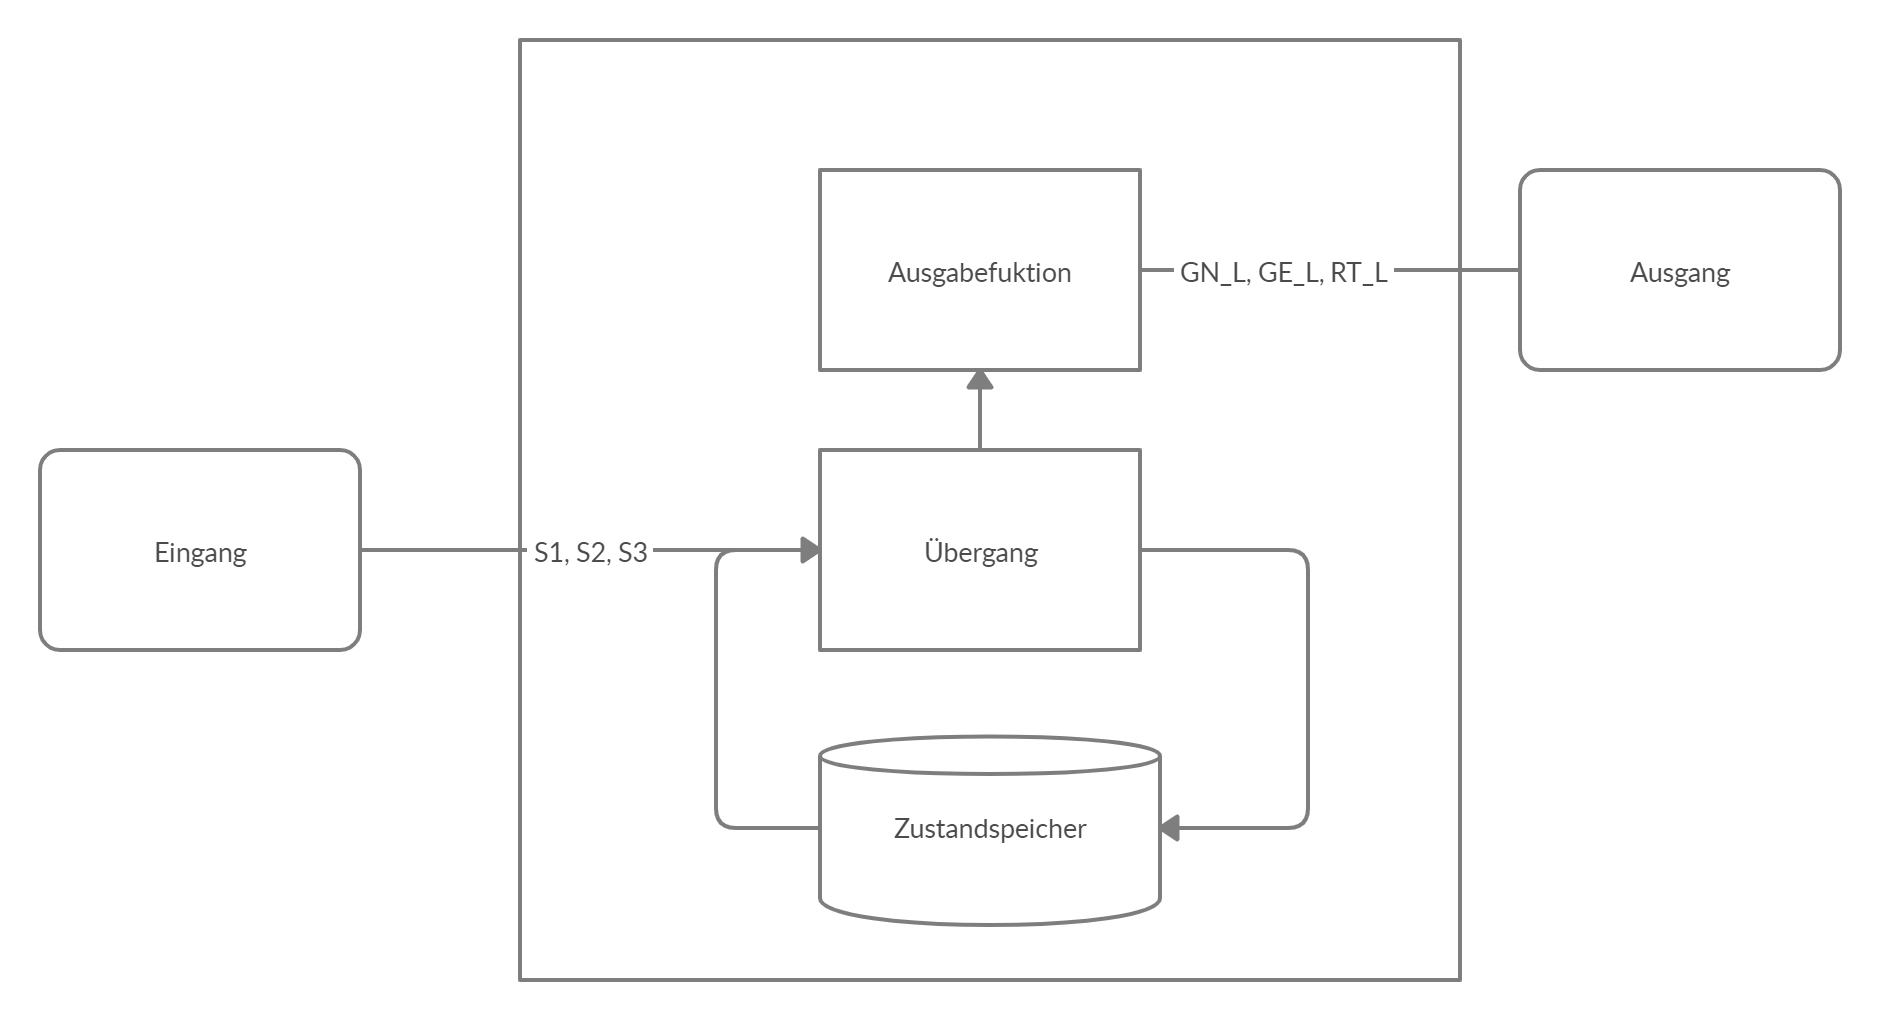
\includegraphics[width=1\textwidth]{img/Blockschalt.png}
        \caption{Blockschalt}
        \label{fig:A1_Block}
    \end{center}
\end{figure}


% grafik einbinden
\begin{figure}[H]
    \begin{center}
        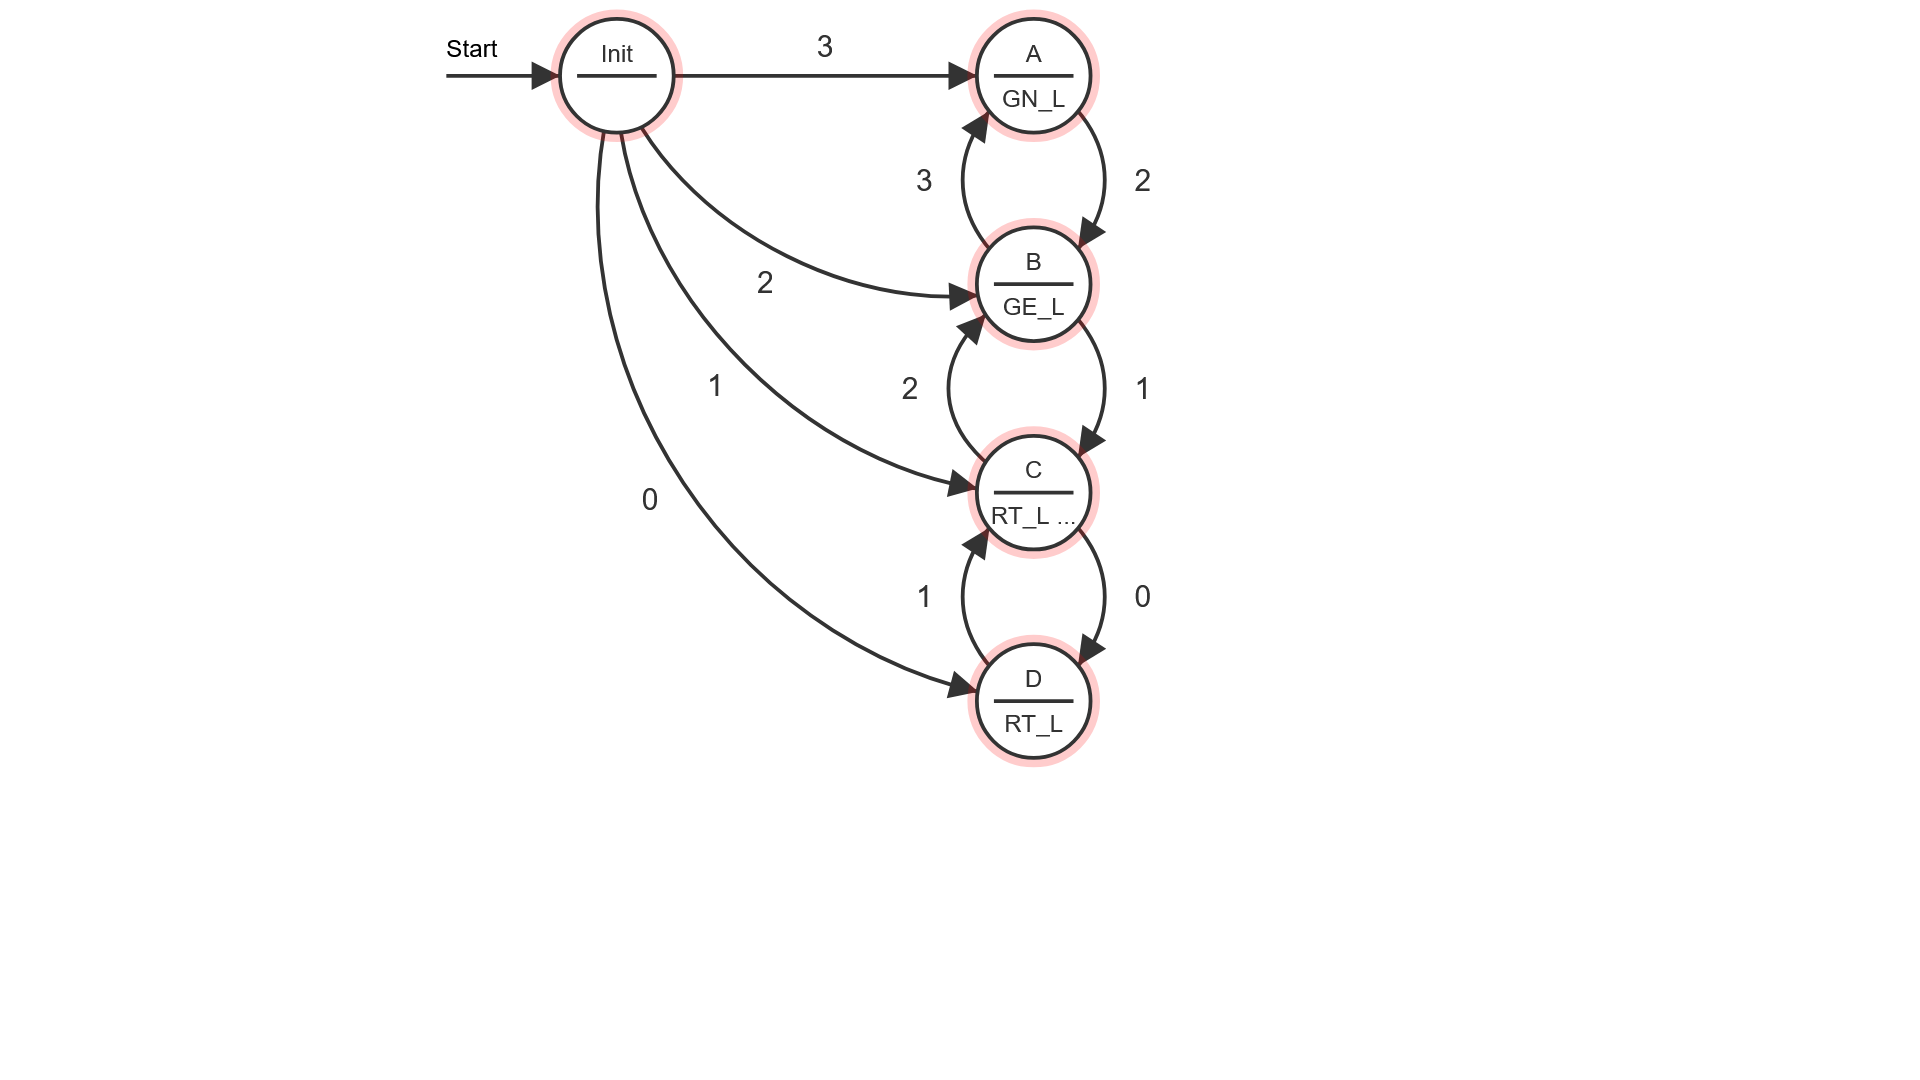
\includegraphics[width=0.6\textwidth]{img/Motortemp2.png}
        \caption{Automatengraph}
        \label{fig:A1_Auto}
    \end{center}
\end{figure}

Das Eingangstupel besteht aus dem Signal der Sensoren der Pumpen. Der Übersichtlichkeit her wurde auf dem Graph nur modelliert, dass eine pumpe ausfallen oder wieder funktionieren kann.
Der Automat kann Zustände auch überspringen, wenn z.B. zwei Pumpen gleichzeitig ausfallen, dies wurde zwecks Übersichtlichkeit nicht eingezeichnet.\\
 
Tupel des Automaten:
Zustände:
\[Q =\{Init, A, B, C, D\}  \]
\[mit \ q_0 = Init \]\\
Eingabealphabet:
\[\Sigma =\{0,1,2,3\} \]\\
Ausgabealphabet:
\[\Omega = \{GN\_L, GE\_L, RT\_L\} \]\\
Ausgabefunktion:
\[\lambda = \lambda  : Q \Rightarrow \Omega: \]
\[  \lambda:GN\_L \Rightarrow \Sigma <= 3 \]
\[  \lambda:GE\_L \Rightarrow 0 < \Sigma <= 2  \]
\[  \lambda:RT\_L \Rightarrow  \Sigma <= 1  \]\\


 \begin{table}[H]
    \centering
    \begin{tabular}{|c|c|c|c|c|c|c|}\hline
    \tbf{$\delta$ (Übergang) $\searrow$} & \tbf{$\Sigma= 0$} & \tbf{$\Sigma= 1$}  & \tbf{$\Sigma= 2$} & \tbf{$\Sigma= 3$} & \tbf{$\Delta$ (Ausgabe)} \\ \hline
    $q_0$ = Init    & D     & C     & B     & A     & GN\_L, GE\_L, RT\_L   \\
    A       & D     & C     & B     & A     & GN\_L                 \\ 
    B       & D     & C     & B     & A     & GE\_L                 \\ 
    C       & D     & C     & B     & A     & GE\_L + RT\_L         \\ 
    D       & D     & C     & B     & A     & RT\_L                 \\ \hline
    \end{tabular} 
    \caption{ Automatentafel}
\end{table}

\newpage





	
\section{Fazit}
insgseamt sieht man hier einen tollen automaten der keinen endzustand hat. und wo es irrelevant ist in welchem zustand er sich befindet. schön

Der automat reagiert wie ein automat lol. er macht das was man ihm sagt.
mehr nicht
fazit ende

	


	\newpage



\end{document}